\documentclass[12pt,a4paper]{article}

% ─── Page Layout ───────────────────────────────────────────────────────────────
\usepackage[a4paper, margin=0.8in, headheight=14pt]{geometry}

% ─── Fonts (XeLaTeX) ───────────────────────────────────────────────────────────
\usepackage{fontspec}
\usepackage{unicode-math}
\setmainfont{TeX Gyre Pagella}
\setmonofont[Scale=0.88]{TeX Gyre Cursor}
\setmathfont{Latin Modern Math}

% ─── Packages ──────────────────────────────────────────────────────────────────
\usepackage{xcolor}
\usepackage{colortbl}
\usepackage{titlesec}
\usepackage{enumitem}
\usepackage{tabularx}
\usepackage{booktabs}
\usepackage{array}
\usepackage{amsmath}
\usepackage{tikz}
\usetikzlibrary{shapes.geometric, arrows.meta, positioning, calc, fit, decorations.pathreplacing}
\usepackage{tcolorbox}
\tcbuselibrary{skins, breakable}
\usepackage{hyperref}
\usepackage{fancyhdr}
\usepackage{graphicx}
\usepackage{microtype}
\hyphenpenalty=10000
\exhyphenpenalty=10000
\sloppy
\usepackage{caption}
\usepackage{setspace}
\usepackage{multirow}
\usepackage{tocloft}

% ─── Q&A helper ────────────────────────────────────────────────────────────────
\newcommand{\Q}[1]{\textbf{#1}\par\noindent\ignorespaces}

% ─── Colour Palette ────────────────────────────────────────────────────────────
\definecolor{myred}{RGB}{196,30,58}
\definecolor{mydark}{RGB}{30,30,50}
\definecolor{mygreen}{RGB}{14,120,80}
\definecolor{myteal}{RGB}{0,130,140}
\definecolor{myamber}{RGB}{180,100,0}
\definecolor{mypurple}{RGB}{100,30,160}
\definecolor{mygray}{RGB}{246,247,249}
\definecolor{mgframe}{RGB}{180,185,200}
\definecolor{watermark}{RGB}{145,150,170}
\definecolor{hdrred}{RGB}{250,232,235}
\definecolor{hdrgreen}{RGB}{220,244,233}
\definecolor{hdrteal}{RGB}{220,242,244}
\definecolor{hdramber}{RGB}{253,242,215}
\definecolor{hdrpurple}{RGB}{238,228,255}
\definecolor{hdrgray}{RGB}{238,240,245}
\definecolor{rowalt}{RGB}{250,251,253}

% ─── Section Formatting ────────────────────────────────────────────────────────
\titleformat{\section}
  {\large\bfseries\color{myred}}{\thesection.}{0.5em}{}
  [\vspace{1pt}{\color{myred}\rule{\linewidth}{0.8pt}}]
\titleformat{\subsection}
  {\normalsize\bfseries\color{myteal}}{\thesubsection}{0.5em}{}
\titlespacing*{\section}{0pt}{18pt}{7pt}
\titlespacing*{\subsection}{0pt}{11pt}{4pt}

% ─── Paragraph ─────────────────────────────────────────────────────────────────
\setlength{\parindent}{0pt}
\setlength{\parskip}{4pt}

% ─── TOC Styling ───────────────────────────────────────────────────────────────
\renewcommand{\cfttoctitlefont}{\large\bfseries\color{myred}}
\renewcommand{\cftaftertoctitle}{\par\noindent{\color{myred}\rule{\linewidth}{0.8pt}}}
\setlength{\cftbeforetoctitleskip}{0pt}
\setlength{\cftaftertoctitleskip}{6pt}
\renewcommand{\cftsecfont}{\normalsize\bfseries\color{mydark}}
\renewcommand{\cftsecpagefont}{\normalsize\bfseries\color{mydark}}
\renewcommand{\cftsecleader}{\cftdotfill{\cftdotsep}}
\setlength{\cftbeforesecskip}{7pt}
\renewcommand{\cftsubsecfont}{\small\color{mydark}}
\renewcommand{\cftsubsecpagefont}{\small\color{mydark}}
\setlength{\cftbeforesubsecskip}{3pt}
\setlength{\cftsubsecindent}{1.4em}

% ─── Table helpers ─────────────────────────────────────────────────────────────
\renewcommand{\arraystretch}{1.45}
\setlength{\tabcolsep}{6pt}
\arrayrulecolor{mydark}
\newcolumntype{B}[1]{>{\small\bfseries\raggedright\arraybackslash}m{#1}}
\newcolumntype{Y}{>{\small\raggedright\arraybackslash}X}
\renewcommand{\tabularxcolumn}[1]{m{#1}}

% ─── Header / Footer ───────────────────────────────────────────────────────────
\pagestyle{fancy}
\fancyhf{}
\fancyhead[L]{\small\color{myred}\textbf{PE-EC603C}\;\color{mydark}--- CMOS VLSI Design}
\fancyhead[R]{\small\color{myteal}\textbf{Module 3 Notes}}
\fancyfoot[C]{\small\color{mydark}\thepage}
\fancyfoot[R]{\small\color{watermark}\textit{\copyright\ Biraj}}
\renewcommand{\headrulewidth}{0.5pt}
\renewcommand{\footrulewidth}{0.3pt}

% ─── Hyperref ──────────────────────────────────────────────────────────────────
\hypersetup{
  colorlinks=true, linkcolor=myteal, urlcolor=myteal,
  pdfauthor={Biraj Sarkar},
  pdftitle={PE-EC603C --- Module 3 Notes}
}

% ─── tcolorbox styles ──────────────────────────────────────────────────────────
\tcbset{
  tikzbox/.style={
    colback=mygray, colframe=mgframe, boxrule=0.6pt, arc=4pt,
    left=8pt, right=8pt, top=6pt, bottom=6pt,
    colbacktitle=mgframe, coltitle=mydark,
    fonttitle=\small\bfseries
  },
  defbox/.style={
    colback=hdrgreen, colframe=mygreen, boxrule=0.8pt, arc=4pt,
    left=9pt, right=9pt, top=6pt, bottom=6pt,
    colbacktitle=mygreen, coltitle=white,
    fonttitle=\small\bfseries
  },
  formulabox/.style={
    colback=hdrteal, colframe=myteal, boxrule=0.8pt, arc=4pt,
    left=9pt, right=9pt, top=7pt, bottom=7pt,
    colbacktitle=myteal, coltitle=white,
    fonttitle=\small\bfseries
  },
  examplebox/.style={
    colback=hdramber, colframe=myamber, boxrule=0.8pt, arc=4pt,
    left=9pt, right=9pt, top=6pt, bottom=6pt,
    colbacktitle=myamber, coltitle=white,
    fonttitle=\small\bfseries
  },
  masonbox/.style={
    colback=hdrpurple, colframe=mypurple, boxrule=0.8pt, arc=4pt,
    left=9pt, right=9pt, top=6pt, bottom=6pt,
    colbacktitle=mypurple, coltitle=white,
    fonttitle=\small\bfseries
  },
  exambox/.style={
    colback=hdrpurple, colframe=mypurple, boxrule=1pt, arc=5pt,
    left=10pt, right=10pt, top=8pt, bottom=8pt,
    colbacktitle=mypurple, coltitle=white,
    fonttitle=\bfseries,
    breakable, title after break={\textbf{Frequently Asked / Viva Questions (contd.)}}}
}
% Make all boxes breakable across pages
\tcbset{breakable}

% ─── TikZ styles ───────────────────────────────────────────────────────────────
\tikzset{
  block/.style={rectangle, draw=myteal, fill=hdrteal,
    text width=2.4cm, align=center, minimum height=0.95cm,
    font=\small, rounded corners=3pt, line width=0.7pt},
  redblock/.style={rectangle, draw=myred, fill=hdrred,
    text width=2.4cm, align=center, minimum height=0.95cm,
    font=\small, rounded corners=3pt, line width=0.7pt},
  greenblock/.style={rectangle, draw=mygreen, fill=hdrgreen,
    text width=2.4cm, align=center, minimum height=0.95cm,
    font=\small, rounded corners=3pt, line width=0.7pt},
  amberblock/.style={rectangle, draw=myamber, fill=hdramber,
    text width=2.4cm, align=center, minimum height=0.95cm,
    font=\small, rounded corners=3pt, line width=0.7pt},
  purpblock/.style={rectangle, draw=mypurple, fill=hdrpurple,
    text width=2.4cm, align=center, minimum height=0.95cm,
    font=\small, rounded corners=3pt, line width=0.7pt},
  sumjunc/.style={circle, draw=myamber, fill=hdramber,
    minimum size=0.62cm, font=\small, line width=0.8pt},
  arrow/.style={-Stealth, thick, color=mydark},
  redarrow/.style={-Stealth, thick, color=myred},
  line/.style={thick, color=mydark}
}

% ═══════════════════════════════════════════════════════════════════════════════
\begin{document}
% ═══════════════════════════════════════════════════════════════════════════════

\begin{center}
  {\LARGE\bfseries\color{myred} PE-EC603C --- CMOS VLSI Design}\\[5pt]
  {\normalsize\color{mydark} Semester VI \quad$\bullet$\quad 3L:0T:0P \quad$\bullet$\quad 3 Credits}\\[3pt]
  {\normalsize\color{myteal}\textbf{Module 3 Exam Notes: VLSI and IC Fabrication Technology}}\\[3pt]
  {\small\color{mydark} CGEC \;$|$\; B.Tech ECE (2023--27) \;$|$\; \textit{Biraj Sarkar}}
\end{center}
\vspace{2pt}
\noindent{\color{myred}\rule{\linewidth}{1.5pt}}
\vspace{2pt}

\hypersetup{linkcolor=mydark}
\tableofcontents
\hypersetup{linkcolor=myteal}
\newpage

% ===============================================================================
\section{Unit Fabrication Processes in VLSI}
% ===============================================================================

IC fabrication involves a sequential series of chemical and physical processing steps performed on a high-purity silicon wafer substrate.

\subsection{Wafer Preparation}
Raw silicon dioxide (sand) is reduced to electronic-grade silicon (EGS). Wafers are cut from a single-crystal ingot grown via the \textbf{Czochralski (CZ) method}, followed by slicing, edge-rounding, grinding, and chemical-mechanical polishing (CMP) to create a defect-free surface.

\subsection{Oxidation}
The process of growing a thin layer of silicon dioxide ($\text{SiO}_2$) on the silicon surface. It is used as a gate oxide, masking layer, and passivation barrier.
\begin{itemize}[leftmargin=*, itemsep=3pt]
  \item \textbf{Dry Oxidation ($\text{Si} + \text{O}_2 \to \text{SiO}_2$):} Performed in pure oxygen gas. Growth is slow, but produces high-density, high-quality oxides. Used for thin gate oxides.
  \item \textbf{Wet Oxidation ($\text{Si} + 2\text{H}_2\text{O} \to \text{SiO}_2 + 2\text{H}_2$):} Performed in water vapor. Growth is very fast, but density is lower. Used for thick field oxides (FOX) or masking layers.
\end{itemize}

\begin{tcolorbox}[defbox, title={\textbf{Deal-Grove Model of Oxidation}}]
The oxide thickness $x_{ox}$ grown over time $t$ is expressed by the quadratic relation:
\begin{equation}
  x_{ox}^2 + A \cdot x_{ox} = B(t + \tau)
\end{equation}
\begin{itemize}[leftmargin=*, itemsep=2.5pt, topsep=2.5pt]
  \item \textbf{Short times (linear regime)}: $x_{ox} \approx \frac{B}{A}(t + \tau)$ (reaction rate-limited).
  \item \textbf{Long times (parabolic regime)}: $x_{ox} \approx \sqrt{B \cdot t}$ (diffusion-limited through existing oxide).
\end{itemize}
\end{tcolorbox}

\subsection{Photolithography}
A process used to transfer geometric patterns from a photo-mask onto the wafer surface.
1. \textbf{Coating}: Apply light-sensitive polymer liquid (\textbf{Photoresist - PR}) on the wafer and spin to distribute uniformly. Soft-bake to drive off solvents.
2. \textbf{Exposure}: Shine UV light through a chrome pattern photo-mask onto the PR layer.
   \begin{itemize}[leftmargin=*, noitemsep, topsep=2pt]
     \item \textbf{Positive PR}: Exposed regions become soluble in developer solution.
     \item \textbf{Negative PR}: Exposed regions polymerize/cross-link, becoming insoluble.
   \end{itemize}
3. \textbf{Development}: Wash away soluble photoresist in developer solution. Hard-bake to solidify the remaining PR pattern.

\subsection{Diffusion \& Ion Implantation}
These processes introduce dopant impurities (boron for p-type, phosphorus/arsenic for n-type) into selective regions of the silicon substrate:
\begin{itemize}[leftmargin=*, itemsep=3.5pt]
  \item \textbf{Diffusion}: High-temperature thermal process ($900^\circ\text{C}$--$1100^\circ\text{C}$). Dopant atoms diffuse isotropically (in all directions, leading to lateral junction spreading beneath the masks) following Fick's laws of diffusion.
  \item \textbf{Ion Implantation}: An energetic beam of dopant ions is accelerated in an electric field ($10$--$500\,\text{keV}$) and directed at the wafer. Ions penetrate vertically, creating a precise, anisotropic dopant profile. This causes lattice damage, requiring high-temperature \textbf{thermal annealing} to restore the crystal structure.
\end{itemize}

\subsection{Deposition (CVD \& PVD)}
Used to grow thin films of materials (polysilicon, silicon nitride, metals) on the wafer surface.
\begin{itemize}[leftmargin=*, itemsep=3pt]
  \item \textbf{Chemical Vapor Deposition (CVD):} Gaseous precursors react chemically at the wafer surface (e.g., thermal decomposition of silane to deposit polysilicon: $\text{SiH}_4 \to \text{Si} + 2\text{H}_2$).
  \item \textbf{Physical Vapor Deposition (PVD):} Physical transfer of atoms (sputtering or vacuum evaporation) from a metal target to the wafer. Used for metallization.
\end{itemize}

\subsection{Etching \& Chemical Mechanical Planarization (CMP)}
\begin{itemize}[leftmargin=*, itemsep=3.5pt]
  \item \textbf{Etching}: Selective removal of material not protected by photoresist.
  \begin{itemize}[leftmargin=*, noitemsep, topsep=2pt]
    \item \textbf{Wet Chemical Etching}: Isotropic, causes undercutting under the mask.
    \item \textbf{Reactive Ion Etching (RIE) / Dry Etching}: Anisotropic, uses gas plasma to etch vertically.
  \end{itemize}
  \item \textbf{CMP}: A chemical slurry and mechanical polishing pad process used to achieve flat, planar surfaces before subsequent lithography steps.
\end{itemize}

\section{CMOS Fabrication Process Flow}

CMOS circuits require the fabrication of both n-channel and p-channel MOSFETs on the same substrate. Since the substrate can only have one doping type (e.g., p-type), a localized well of the opposite type (e.g., n-well) must be created to house the complementary device.

\subsection{n-Well CMOS Process Flow Steps}
Starting with a p-type substrate:
1. \textbf{Well Formation}: Lithography and ion implantation of phosphorus/arsenic to create the \textbf{n-well region} (where pMOS transistors will be placed). Drive-in anneal.
2. \textbf{Active Area Definition}: Deposit silicon nitride ($\text{Si}_3\text{N}_4$) as a mask, pattern it, and grow thick \textbf{Field Oxide (FOX)} via local oxidation of silicon (LOCOS) to isolate active regions.
3. \textbf{Threshold Adjust Implants}: Implantation of boron to adjust the threshold voltages of both nMOS and pMOS devices.
4. \textbf{Gate Oxide Growth}: Grow high-quality, ultra-thin dry gate oxide layer ($\text{SiO}_2$).
5. \textbf{Polysilicon Gate Formation}: Deposit polysilicon via CVD, pattern it with lithography, and etch to form the gate electrodes.
6. \textbf{Source/Drain Implantation (Self-Aligned Gates)}:
   \begin{itemize}[leftmargin=*, noitemsep, topsep=2pt]
     \item Implant arsenic/phosphorus ($n^+$) to form nMOS source/drain and the n-well body contact tap. The polysilicon gate acts as a self-aligned mask for the channel.
     \item Implant boron ($p^+$) to form pMOS source/drain and the p-substrate body contact tap.
   \end{itemize}
7. \textbf{Interlevel Dielectric (ILD) Deposition}: Deposit thick insulating oxide layer, etch contact holes.
8. \textbf{Metallization}: Deposit metal (aluminum/copper) via PVD, pattern, and etch to form interconnects.

\begin{tcolorbox}[tikzbox, title={CMOS Inverter Fabrication Cross-Section}]
\centering
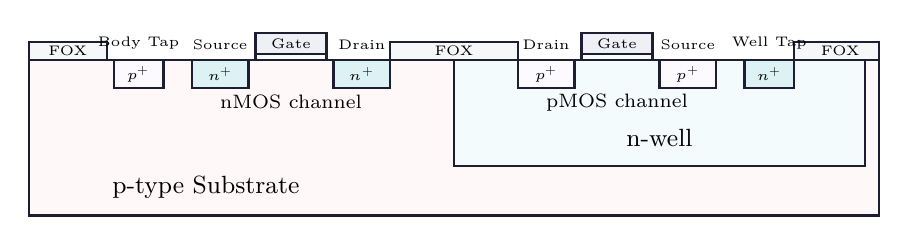
\begin{tikzpicture}[scale=0.9, thick, font=\small]
  % P-type Substrate
  \draw[draw=mydark, fill=hdrred!30] (-6.0, -2.2) rectangle (6.0, 0);
  \node at (-3.5, -1.8) {p-type Substrate};
  
  % N-well (on the right)
  \draw[draw=mydark, fill=hdrteal!30] (0.0, -1.5) rectangle (5.8, 0);
  \node at (2.9, -1.1) {n-well};
  
  % Field Oxide (FOX) Isolation blocks at surface
  \draw[draw=mydark, fill=mygray] (-6.0, 0) rectangle (-4.9, 0.25);
  \draw[draw=mydark, fill=mygray] (-0.9, 0) rectangle (0.9, 0.25);
  \draw[draw=mydark, fill=mygray] (4.8, 0) rectangle (6.0, 0.25);
  \node[font=\tiny] at (-5.45, 0.12) {FOX};
  \node[font=\tiny] at (0, 0.12) {FOX};
  \node[font=\tiny] at (5.45, 0.12) {FOX};
  
  % nMOS active implants (left)
  \draw[draw=mydark, fill=hdrpurple!20] (-4.8, -0.4) rectangle (-4.1, 0);
  \node[font=\tiny] at (-4.45, -0.2) {$p^+$};
  \draw[draw=mydark, fill=hdrteal] (-3.7, -0.4) rectangle (-2.9, 0);
  \node[font=\tiny] at (-3.3, -0.2) {$n^+$};
  \draw[draw=mydark, fill=hdrteal] (-1.7, -0.4) rectangle (-0.9, 0);
  \node[font=\tiny] at (-1.3, -0.2) {$n^+$};
  \node[font=\scriptsize] at (-2.3, -0.6) {nMOS channel};
  
  % pMOS active implants (right)
  \draw[draw=mydark, fill=hdrpurple!20] (0.9, -0.4) rectangle (1.7, 0);
  \node[font=\tiny] at (1.3, -0.2) {$p^+$};
  \draw[draw=mydark, fill=hdrpurple!20] (2.9, -0.4) rectangle (3.7, 0);
  \node[font=\tiny] at (3.3, -0.2) {$p^+$};
  \draw[draw=mydark, fill=hdrteal] (4.1, -0.4) rectangle (4.8, 0);
  \node[font=\tiny] at (4.45, -0.2) {$n^+$};
  \node[font=\scriptsize] at (2.3, -0.6) {pMOS channel};
  
  % Gate Oxides and Polysilicon Gates
  % nMOS Gate
  \draw[draw=mydark, fill=hdrgreen!20] (-2.8, 0) rectangle (-1.8, 0.08); % Oxide
  \draw[draw=mydark, fill=hdrgray] (-2.8, 0.08) rectangle (-1.8, 0.38); % Gate
  \node[font=\tiny] at (-2.3, 0.23) {Gate};
  
  % pMOS Gate
  \draw[draw=mydark, fill=hdrgreen!20] (1.8, 0) rectangle (2.8, 0.08); % Oxide
  \draw[draw=mydark, fill=hdrgray] (1.8, 0.08) rectangle (2.8, 0.38); % Gate
  \node[font=\tiny] at (2.3, 0.23) {Gate};

  % Text labels for implants
  \node[above, font=\tiny] at (-4.45, 0) {Body Tap};
  \node[above, font=\tiny] at (-3.3, 0) {Source};
  \node[above, font=\tiny] at (-1.3, 0) {Drain};
  \node[above, font=\tiny] at (1.3, 0) {Drain};
  \node[above, font=\tiny] at (3.3, 0) {Source};
  \node[above, font=\tiny] at (4.45, 0) {Well Tap};
\end{tikzpicture}
\end{tcolorbox}

\subsection{p-Well and Twin-Tub CMOS Processes}
\begin{itemize}[leftmargin=*, itemsep=3.5pt]
  \item \textbf{p-Well Process}: Starts with an n-type substrate. nMOS transistors are created inside a fabricated p-well, while pMOS transistors are fabricated directly in the n-substrate.
  \item \textbf{Twin-Tub Process}: Starts with a high-resistivity wafer containing an epitaxial layer. Both an n-well (tub) and a p-well (tub) are fabricated separately to optimize nMOS and pMOS channel profiles independently, eliminating threshold voltage offsets and minimizing latch-up risk.
\end{itemize}

\newpage
% ===============================================================================
% MANDATORY QUICK REVISION PAGE
% ===============================================================================
\begin{center}
  {\large\bfseries\color{myred} Quick Revision --- Module 3}\\[3pt]
  {\small\color{mydark} VLSI and IC Fabrication Technology $|$ PE-EC603C}
\end{center}
\noindent{\color{myred}\rule{\linewidth}{1.2pt}}
\vspace{4pt}

\begin{tcolorbox}[formulabox, title={\textbf{Key Fabrication Equations}}]
$$\text{Deal-Grove Model:} \quad x_{ox}^2 + A \cdot x_{ox} = B(t + \tau)$$
$$\text{Linear Oxide growth rate (thin):} \quad \frac{dx_{ox}}{dt} \approx \frac{B}{A} \qquad \text{Parabolic rate (thick):} \quad \frac{dx_{ox}}{dt} \approx \frac{B}{2x_{ox}}$$
$$\text{Fick's Second Law of Diffusion:} \quad \frac{\partial C(x,t)}{\partial t} = D \frac{\partial^2 C(x,t)}{\partial x^2}$$
\end{tcolorbox}

\begin{tcolorbox}[defbox, title={\textbf{One-Line Definitions}}]
\begin{itemize}[leftmargin=*, itemsep=2.5pt, topsep=0pt]
  \item \textbf{Czochralski Method:} Silicon crystal growth technique pulling single-crystal ingots from a liquid melt.
  \item \textbf{Dry Oxidation:} Oxidation utilizing pure oxygen gas, producing thin, highly uniform gate dielectric layers.
  \item \textbf{Wet Oxidation:} Oxidation utilizing steam water vapor, growing thick field oxides (FOX) rapidly.
  \item \textbf{Photoresist:} Light-sensitive organic polymer liquid used to transfer photomask geometric patterns.
  \item \textbf{Ion Implantation:} Anisotropic process accelerating dopant ions at high fields to target precise vertical depth profiles.
  \item \textbf{Self-Aligned Gate:} Technique where polysilicon gates act as masks for source/drain implants, preventing overlap offsets.
  \item \textbf{Twin-Tub CMOS:} Fabricating both n-well and p-well regions on epitaxial layers to optimize both transistor profiles.
\end{itemize}
\end{tcolorbox}

\begin{tcolorbox}[exambox, title={\textbf{Frequently Asked / Viva Questions}}]
\begin{enumerate}[topsep=0pt, label=\textbf{Q\arabic*.}, itemsep=5pt]
  \item \Q{Compare dry oxidation and wet oxidation in terms of growth rate, density, and application.}
    Dry oxidation uses pure oxygen; its growth rate is slow but it produces high-density, high-quality oxides, making it suitable for thin gate oxides. Wet oxidation uses steam; its growth rate is very fast but it yields lower density, making it suitable for thick field isolation oxides (FOX).
  \item \Q{Explain the difference between positive and negative photoresists.}
    In positive photoresists, exposure to UV light breaks down chemical bonds, making the exposed region highly soluble in the developer. In negative photoresists, UV exposure causes cross-linking, making the exposed region insoluble while unexposed regions wash away.
  \item \Q{Why is ion implantation preferred over thermal diffusion for doping?}
    Ion implantation is highly anisotropic, allowing precise independent control of both dose (total quantity of atoms) and depth (controlled by acceleration energy) with minimal lateral spreading under masks. Thermal diffusion is isotropic and spreads laterally.
  \item \Q{What is the Deal-Grove model and what are its two limiting regimes?}
    The Deal-Grove model describes the kinetics of thermal oxidation. The two limiting regimes are the linear regime (for thin oxides, reaction-rate limited at the silicon interface, $x_{ox} \propto t$) and the parabolic regime (for thick oxides, diffusion-limited through the existing $\text{SiO}_2$ layer, $x_{ox} \propto \sqrt{t}$).
  \item \Q{What is thermal annealing and why is it necessary after ion implantation?}
    During ion implantation, high-energy dopant ions bombard the silicon lattice, knocking atoms out of position and damaging the crystal structure. Thermal annealing heats the wafer (typically $900^\circ\text{C}$ to $1000^\circ\text{C}$) to repair the crystal lattice and electrically activate the dopants.
  \item \Q{Explain the term "Self-Aligned Gate" process.}
    In this process, the polysilicon gate is patterned first. During the subsequent source/drain ion implantation, the gate itself acts as a mask protecting the channel region. This guarantees perfect alignment of the source/drain junctions with the gate edges, eliminating overlap capacitances.
  \item \Q{What is the function of the body tap ($p^+$ in p-substrate) and well tap ($n^+$ in n-well)?}
    The body tap connects the p-substrate to the lowest potential (GND) and the well tap connects the n-well to the highest potential ($V_{DD}$). This keeps the parasitic p-substrate/n-well p-n junctions reverse-biased, preventing latch-up.
  \item \Q{What is Local Oxidation of Silicon (LOCOS) and what is its drawback?}
    LOCOS is a selective oxidation process using silicon nitride masks to grow thick field oxide (FOX) for isolating adjacent devices. Its drawback is the lateral diffusion of oxygen under the nitride mask, forming a sloped oxide region called the "bird's beak", which wastes active area.
  \item \Q{What is Shallow Trench Isolation (STI)?}
    STI is an isolation technique that replaces LOCOS in sub-micron technologies. It involves etching a shallow trench between active areas, filling it with deposited oxide (CVD), and planarizing it using CMP. It eliminates the bird's beak effect.
  \item \Q{Describe the Twin-Tub CMOS process and its benefits.}
    The Twin-Tub process creates both an n-well and a p-well tub inside a high-resistivity epitaxial layer. This allows the doping profiles, threshold voltages, and body effects of nMOS and pMOS transistors to be optimized independently.
\end{enumerate}
\end{tcolorbox}

\end{document}
